\chapter[Capítulo 4]{Capítulo 4}
\label{ch:cap4}
\lipsum[3-5]

\section{Seção}

\lipsum[1-2]

\subsection{Subseção}
\lipsum[3-5]

\section{Seção 2}\label{secao2}

O SHAPE é a sigla em inglês para \textit{Symbolic Hierarchical Automated Reliability and Performance Evaluator}. Veja a  \autoref{fig:sharpe}.

\begin{figure}[!h]
	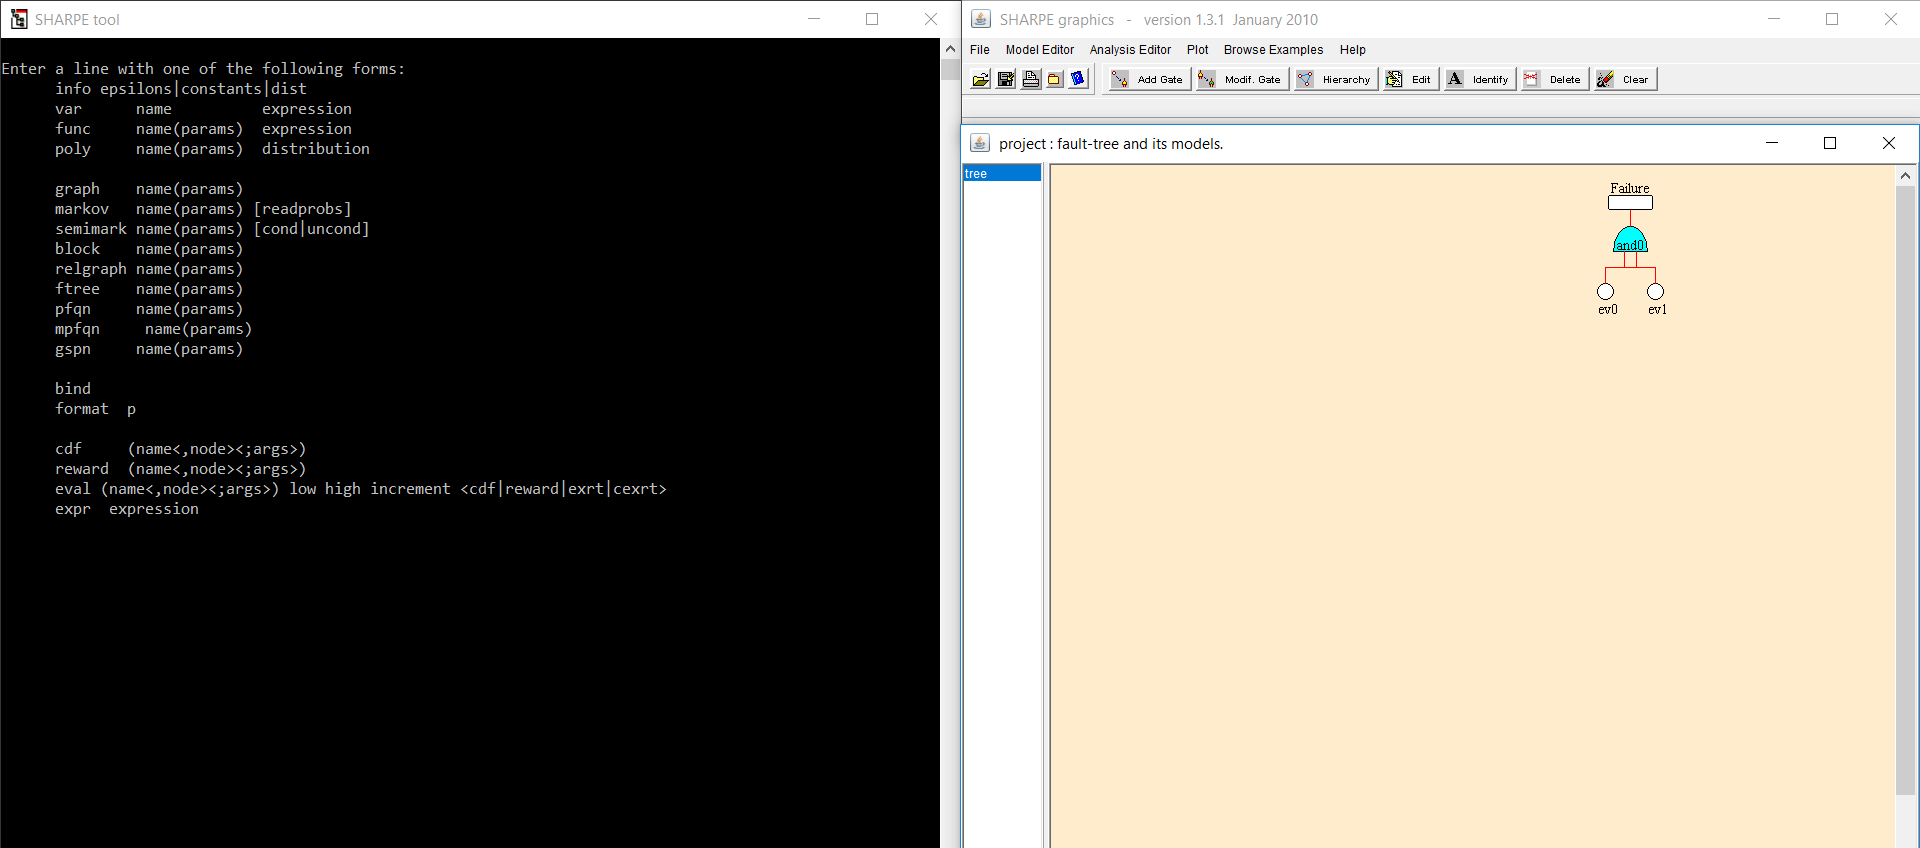
\includegraphics[width=1.0\textwidth, keepaspectratio=true]{sharpe}
	\centering
	\caption[\textit{Print screen} do SHARPE em linha de comando e em interface gráfica.]{\textit{Print screen} do SHARPE em linha de comando e em interface gráfica.}
	\fonte{Elaborada pela autora.}
	\label{fig:sharpe}
\end{figure}